\documentclass[../../main.tex]{subfiles}

\begin{document}

\label{sec:abbildungen_verkettung}

Funktionen ordnen Argumenten, die aus ihrer Definitionsmenge kommen, ihr jeweiliges Bild zu. Auf diese Weise erhält man bei einer Funktion $f\colon U\rightarrow V$ Bilder aus der Menge $V$. Wie im folgenden Beispiel kommt es manchmal vor, dass nach Anwendung einer Funktion direkt eine zweite Funktion angewandt werden soll.

\begin{example}{}
    \parpic[r]{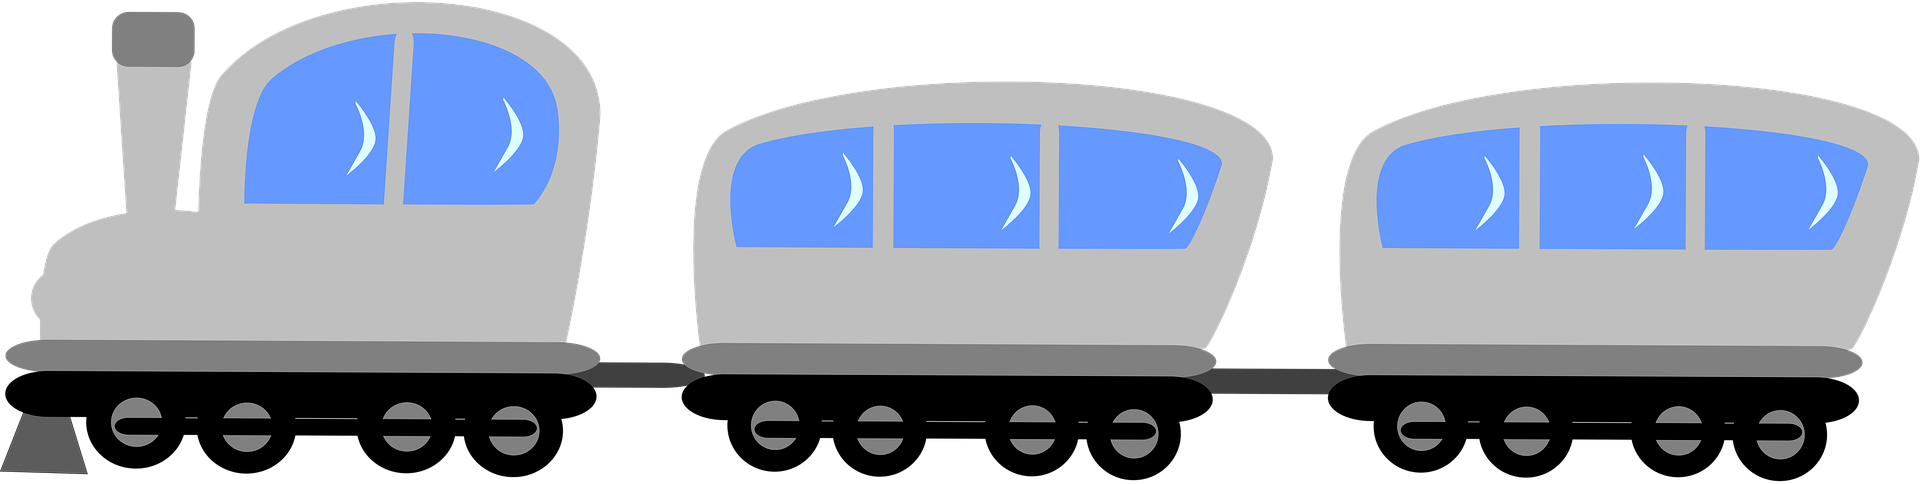
\includegraphics[width=.33\textwidth]{images/train.png}}
    Eine Gruppe von sechs Freunden möchte sich in Hamburg-Niendorf treffen. Zwei von ihnen wohnen außerhalb von Hamburg. Deswegen steigen sie zunächst in einen Zug, der sie zum Hamburger Hauptbahnhof fährt. Nach der Ankunft steigen die beiden um und fahren mit der U-Bahn weiter, bis sie ihre Freunde im Stadtteil Niendorf treffen.
    
    \picskip{0}
    Der Zug transportiert alle, die bis zur Endstation fahren, zum Hauptbahnhof (und beschreibt auf diese Weise eine Funktion $\textsc{ZugNachHamburg}$, die allen Orten, an denen Gäste einsteigen, den Ort \emph{Hamburg Hbf.} zuordnet). Die Straßenbahn nach Niendorf transport die beiden Freunde vom Hauptbahnhof nach Niendorf (also beschreibt sie eine Funktion $\textsc{BahnNachNiendorf}$, die dem Ort \emph{Hamburg Hbf.} den Stadtteil \emph{Niendorf} zuordnet).
    
    Wenn einer der Freunde in Itzehoe (einer Stadt nördlich von Hamburg) in den Zug nach Hamburg steigt und dann in die U-Bahn, dann gelangt er nach Niendorf. Auf seinen Ausgangsort \emph{Itzehoe} hat er erst die Funktion $\textsc{ZugNachHamburg}$ angewandt ($\textsc{ZugNachHamburg}(\emph{Itzehoe})=\emph{Hamburg Hbf.}$) und anschließend durch das Einsteigen in die Straßenbahn die Funktion $\textsc{BahnNachNiendorf}$ genutzt, um nach Niendorf zu kommen ($\textsc{BahnNachNiendorf}(\emph{Hamburg Hbf.})=\emph{Niendorf}$).
\end{example}

Bei der \textbf{Verkettung} (auch \emph{Hintereinanderausführung} oder \emph{Komposition}) von Funktionen werden Argumente mithilfe einer Funktion auf ihr Bild abgebildet (so, wie du das bereits aus den letzten Abschnitten kennst) und anschließend wird das erhaltene Bild direkt in eine zweite Funktion eingesetzt und seinerseits einem Bild zugeordnet. Auf diese Weise wird jedes Element aus der Definitionsmenge der ersten Funktion -- mit einem Zwischenschritt -- einem Element aus der Zielmenge der zweiten Funktion zugeordnet.

\begin{example}{}
    Der Freund, der aus Itzehoe nach Niendorf gefahren ist, hat zwei Funktionen hintereinander ausgeführt, also verkettet. Er ist erst mit dem Zug nach Hamburg gefahren und anschließend mit der U-Bahn zu seinem Ziel in Niendorf. Mathematisch aufgeschrieben gilt \[\textsc{BahnNachNiendorf}(\colorbrace{\textsc{ZugNachHamburg}(\emph{Itzehoe})}{\emph{Hamburg Hbf.}})=\emph{Niendorf}.\]
\end{example}

Mathematisch funktioniert die Verkettung von Funktionen so, dass man ein Argument $x$ zunächst benutzt, um $f(x)$ zu berechnen, d.h. um das Bild zu erhalten, das $f$ ihm zuordnet. Anschließend setzt man dieses Ergebnis in eine Funktion $g$ ein. Man berechnet also $g(f(x))$. $f(x)$ wird an dieser Stelle als Argument für $g$ verwendet.

Zwei Funktionen zu verketten, klappt nur dann, wenn die zweite Funktion etwas mit den Ergebnissen der ersten anfangen kann (also für sie definiert ist). Im folgenden Bild siehst du, wie die zweite Funktion genau dort ansetzt, wo die erste aufhört. Dabei teilen sich beide Funktionen eine Menge: Die zweite Funktionen nutzt die Zielmenge der ersten als ihre Definitionsmenge.

\parpic[r]{
    \begin{tikzpicture}[scale=.75]
        \draw[grayset] (-1.5,0) ellipse (0.7cm and 2cm);
        \draw[grayset] (1.5,0) ellipse (0.7cm and 2cm);
        \draw[grayset] (4.5,0) ellipse (0.7cm and 2cm);
    
        \node[red] (x1) at (-1.5,0.7) {$\bullet$};
        %\node (x2) at (-1.5,-0.2) {$\bullet$};
        \node (x3) at (-1.5,-1.1) {$\bullet$};
        \node (y1) at (1.5,0.7) {$\bullet$};
        %\node (y2) at (1.6, 0) {$\bullet$};
        \node[violet] (y3) at (1.5,-1.2) {$\bullet$};
        \node (z1) at (4.5,1.2) {$\bullet$};
        \node (z2) at (4.5,0.4) {$\bullet$};
        \node (z3) at (4.5,-0.4) {$\bullet$};
        \node[blue] (z4) at (4.5,-1.2) {$\bullet$};
    
        \draw[red, ->] (x1) -- (y3);
        %\draw[->] (x2) to[bend right] (y1);
        \draw[red, ->] (x3) to[bend left] (y1);
    
        \draw[blue, ->] (y1) to (z1);
        \draw[blue, ->] (y3) -- (z4);
    
        \draw[black!30, ->] (x1) to (z4);
        %\draw[black!30, ->] (x2) -- (z3);
        \draw[black!30, ->] (x3) -- (z1);
    
        \node[red] at (0,-1) {$f$};
        \node[blue] at (3,-1) {$g$};
        %\node[black!30] at (3,-1.7) {$g\circ f$};
    \end{tikzpicture}
}

Ein Element der links dargestellten Menge kann mit der eingezeichneten Funktion $f$ in ein Element der mittleren Menge übersetzt werden (z.B. kann das rote dem violetten Element zugeordnet werden). Das violette Element kann mithilfe der zweiten eingezeichneten Funktion $g$ einem Element der rechten Menge zugeordnet werden, und zwar dem blauen. Das heißt, dass das rote Element insgesamt mit einem Zwischenschritt dem blauen zugeordnet wird, wenn man erst die linke und dann die rechte Funktion anwendet. Dafür hat man zunächst $f(x)$ berechnet und das Ergebnis anschließend in die Funktion $g$ eingesetzt, also $g(f(x))$ berechnet. Die Verkettung ordnet einem Element der linken Menge also direkt ein Element der ganz rechten Menge zu -- so, wie es durch die grauen Pfeile zu sehen ist.

So ist es möglich, dass -- wie an einem Fließband in einer Fabrik -- erst die Funktion $f$ ein Argument erhält und es in ein Bild übersetzt, mit dem $g$ weiterarbeiten kann. Anschließend erhält $g$ dieses Bild und verarbeitet es weiter.

\begin{example}{}
    \parpic[r]{
        
\includegraphics[height=4.2cm]{images/statue_of_liberty.png}
    }
    
    Bei einer Reise in die USA, in denen man mit der Währung Dollar bezahlt, kann man als Europäer natürlich nicht mit Euro bezahlen. Wer dorthin reist, wechselt deshalb vorher etwas Geld, das er für die Reise einplant, in Dollar.
 
    Mit diesem Geld ist es anschließend unter anderem möglich, vor Ort Essen in Restaurants zu kaufen sowie den Eintritt zu Sehenswürdigkeiten und anderen Touristenattraktionen zu bezahlen. Wir gehen nun davon aus, dass von dem Geld Tickets für den Besuch der Freiheitsstatue gekauft werden sollen (Preis: 40\,\$).

    Für einen USA-Urlaub wechselt man also erst seine Euro in Dollar und anschließend die Dollar in Eintrittskarten, Verpflegung und ähnliches. 
    
    \begin{center}
        \begin{tikzpicture}
            \draw[black!25,fill=black!10] (-1.5,0) circle[radius=6mm];
            \draw[black!25,fill=black!10] (0,0) circle[radius=6mm];
            \draw[black!25,fill=black!10] (1.5,0) circle[radius=6mm];
            %node content
            \node[yellow!70!black] at (-1.5,0) {\euro};
            \node[yellow!70!black] at (0,0) {\$};
            \node[yellow!70!black] at (1.5,0) {
\includegraphics[height=10mm]{images/statue_of_liberty.png}};
            %connection lines
            \draw[very thick,black!40,->] (-1,0) to[bend left] (-0.5,0);
            \draw[very thick,black!40,->] (0.5,0) to[bend left] (1,0);
        \end{tikzpicture}
    \end{center}

    Das Wechseln von Euro in Dollar können wir einfach durch eine Funktion beschreiben. Angenommen, der Wechselkurs liegt bei $1.20\,\$$ pro Euro. Dann ordnet die Funktion $\textsc{Dollar}\colon\Real\rightarrow\Real$ mit der Zuordnungsvorschrift 
    \[\textsc{Dollar}(x)=1.2x\] 
    dem investierten Betrag in Euro zu, wie viele Dollar man dafür erhält. Es gilt beispielsweise $\textsc{Dollar}(5)=6$, weil man 6 Dollar für 5 Euro erhalten würde.
    
    Die Funktion $\textsc{TicketsFürDollar}\colon\Real\rightarrow\Integer$ könnte nun beschreiben, wie viele Tickets man für einen bestimmten Betrag (in Dollar) kaufen kann.

    Möchte man nun wissen, wie viele Tickets für die Freiheitsstatue für 100\,€ erhältlich sind, muss man diesen Betrag zunächst in Dollar umrechnen (mithilfe der Funktion $\textsc{Dollar}$). Es gilt $\textsc{Dollar}(100)=120$. 
    
    Anschließend verrät die Funktion $\textsc{TicketsFürDollar}$, dass man $3$ Tickets kaufen kann, weil man die eben erhaltene $120$ einsetzt und $\textsc{TicketsFürDollar}(120)=3$ gilt.
    
    Wir haben erst $\textsc{Dollar}(100)$ und dann $\textsc{TicketsFürDollar}(120)$ berechnet. Die $120$ ist genau das Ergebnis von $\textsc{Dollar}(100)$. Also ist \[\textsc{TicketsFürDollar}(120)=\textsc{TicketsFürDollar}(\colorbrace{\textsc{Dollar}(100)}{=120}).\]
    
    Um zu berechnen, wie viele Tickets wir für $x$ Euro bekommen, berechnen wir also $\textsc{TicketsFürDollar}(\textsc{Dollar}(x))$.
\end{example}

Zwei Funktionen $f$ und $g$ nacheinander anzuwenden, kann sich manchmal als sinnvoll erweisen, wenn man mit einfachen Zwischenschritten zu einem bestimmten Ergebnis kommt, statt eine kompliziertere Funktion in einem Schritt zu berechnen.

\begin{example}{}
    Wenn du im Kopf für eine bestimmte Zahl $x$ den Wert $3x+2$ ausrechnen möchtest, dann kannst du das nicht sinnvoll in einem Schritt tun. Stattdessen wirst du dir erst überlegen, was $3x$ ist. Anschließend wirst du $2$ zum Ergebnis addieren. In einem ersten Schritt berechnest du also die Funktion $f(x)=3x$, die die Addition von $2$ zunächst ignoriert.
    
    Nachdem du weißt, welchen Wert $3x$ hat, addierst du darauf $2$. Mit der Funktion $g(x)=x+2$ tust du genau das. Führst du beide Funktionen hintereinander aus, berechnest du \[g(f(x))=g(3x)=3x+2,\] also genau das, was du berechnen wolltest -- nur mit einem Zwischenschritt.
    
    Für $x=5$ gilt zum Beispiel $f(5)=3\cdot 5=15$ und $g(f(5))=g(15)=15+2=17$. Natürlich ist auch \[\colorbrace{\colorobrace{3\cdot 5}{f(5)}+2}{g(f(5))}=17.\]
\end{example}

Gerade im letzten Beispiel hast du gesehen, dass auch die Verkettung von zwei Funktionen selbst wieder eine Funktionen ist. Jedes Argument für $f$ wird eindeutig erst einem Argument für $g$ und dann dem Bild, das $g$ produziert, zugewiesen. Die Funktion $g(f(x))$ kann daher selbst als eine Funktion definiert werden. Sie wird die \textbf{Verkettung} oder die \textbf{Komposition} von $f$ und $g$ genannt.

\begin{definition}{Verkettung von Funktionen}
    Es seien $U,V,W$ Mengen und $f\colon U\rightarrow V$ sowie $g\colon V\rightarrow W$ Funktionen.
    
    Die Funktion $g\circ f\colon U\rightarrow W$ mit \[x\mapsto (g\circ f)(x)\coloneqq g(f(x))\] heißt die \textbf{Verkettung} von $f$ und $g$.
\end{definition}

Die Funktion $g\circ f$ ordnet ihre Argumente auf demjenigen Element zu, das man erhält, wenn man erst $f$ und dann $g$ anwendet. Hierbei sollte man sich nicht davon verwirren lassen, dass das $g$ links steht -- das $f$ wird trotzdem zuerst angewandt, denn es befindet sich bei der Schreibweise $g(f(x))$ innen. Die Schreibweise $g\circ f$ aus dieser Definition kann man als \enquote{$g$ verkettet mit $f$} oder \enquote{$g$ Kringel $f$} lesen.

Die Reihenfolge, in der man $f$ und $g$ anwendet, ist für Verkettungen sehr wichtig. Einerseits kann es sein, dass du, wenn du erst $g$ anwendest, überhaupt kein Bild erhältst, das in der Definitionsmenge von $f$ liegt. Es ist aber auch selbst dann, wenn die Definitions- und Zielmengen dennoch zu einander passen, nicht egal, in welcher Reihenfolge du die Funktion anwendest (wie im nächsten Beispiel zu sehen ist).

\begin{example}{}
    Im letzten Beispiel haben wir gesehen, dass $g(f(x))=3x+2$ ist. Die Verkettung dieser beiden Funktionen $g\circ f$ ist die Funktion $(g\circ f)(x)=3x+2$.
    
    Es gilt hingegen aber $(f\circ g)(x)=f(g(x))=f(x+2)=3(x+2)=3x+6$. Die Reihenfolge, in der man $f$ und $g$ anwendet, ist also sehr wichtig und verändert die Funktion, die man bei der Verkettung erhält.
\end{example}

\begin{nutshell}{Verkettung von Funktionen}
    \parpic[r]{\begin{tikzpicture}[scale=.6]
    \draw[grayset] (-1.5,0) ellipse (0.7cm and 2cm);
    \draw[grayset] (1.5,0) ellipse (0.7cm and 2cm);
    \draw[grayset] (4.5,0) ellipse (0.7cm and 2cm);

    \node (x1) at (-1.5,0.7) {$\bullet$};
    \node (x2) at (-1.5,-0.2) {$\bullet$};
    \node (x3) at (-1.5,-1.1) {$\bullet$};
    \node (y1) at (1.5,0.7) {$\bullet$};
    \node (y2) at (1.5,-0.2) {$\bullet$};
    \node (y3) at (1.5,-1.2) {$\bullet$};
    \node (z1) at (4.5,1.2) {$\bullet$};
    \node (z2) at (4.5,0.4) {$\bullet$};
    \node (z3) at (4.5,-0.4) {$\bullet$};
    \node (z4) at (4.5,-1.2) {$\bullet$};

    \draw[->] (x1) -- (y3);
    \draw[->] (x2) to[bend right] (y1);
    \draw[->] (x3) to[bend right] (y2);
    
    \draw[->] (y1) -- (z3);
    \draw[->] (y2) -- (z1);
    \draw[->] (y3) -- (z4);
    
    \node at (0,1) {$f$};
    \node at (3,1) {$g$};
\end{tikzpicture}}
    Zwei Funktionen $f$ und $g$, bei denen $f$ seine Argumente in die Definitionsmenge von $g$ abbildet, können hintereinander angewandt werden. Dafür bildet man ein Element $x$ der Definitionsmenge von $f$ erst mit $f$ und das Ergebnis $f(x)$ dann mit $g$ ab. Man berechnet also $g(f(x))$.
      
    \picskip{0} 
    Die Funktion, die jedes Element aus der Definitionsmenge von $f$ auf das Element der Zielmenge von $g$ abbildet, das man erhält, wenn man erst $f$ und dann $g$ anwendet, heißt \textbf{Verkettung} von $f$ und $g$. Sie wird geschrieben als $g\circ f$. Es gilt also $(g\circ f)(x)=g(f(x))$.
\end{nutshell}

\end{document}